\documentclass{article}
\usepackage[utf8]{inputenc}
\usepackage[margin = 0.8in]{geometry}
\usepackage{graphicx}
\usepackage{amsmath, amssymb}
\usepackage{subcaption}
\usepackage{multirow}
\usepackage{mathtools}
\usepackage{float}
\usepackage{pythonhighlight}


\title{Project 6 - INS/GNSS Integration}
\author{Keith Chester}

\begin{document}
\maketitle


In this assignment we are looking at integrating our previous UKF implementation with an INS/GNSS model. Specifically, we are looking at two possible approaches - a Feedback (FB) model, and a Feed Forward (FF) model. The primary difference is within the state, wherein our FB model state is:

\begin{equation}
    x = \begin{bmatrix} L \\ \lambda \\ h \\ \phi \\ \theta \\ \psi \\ V_N \\ V_E \\ V_D \\ e_L \\ e_\lambda \\ e_h \end{bmatrix}
\end{equation}

...wherein our FF model state is:

\begin{equation}
    x = \begin{bmatrix} L \\ \lambda \\ h \\ \phi \\ \theta \\ \psi \\ V_N \\ V_E \\ V_D \\ b_{a_x} \\ b_{a_y} \\ b_{a_z} \\ b_{g_x} \\ b_{g_y} \\ b_{g_z} \end{bmatrix}
\end{equation}

...wherein our biases are calculated as the linear difference between latitude and longitude and the estimated state.

\section*{Propagation Model}

In this UKF model, we follow the propagation model of applying an attitude update, a velocity update, and finally a position update.

\subsection*{Attitude Update}

Our attitude update starts with $\omega_E$, which is defined as the rotation of the the earth in radians a second - $7.292 \times 10^{-5} \frac{rad}{s}$. We form a screw rotation matrix $\Omega^i_e$ as:

\begin{equation}
    \Omega^i_e = \begin{bmatrix} 0        & -\omega_E & 0 \\
                \omega_E & 0         & 0 \\
                0        & 0         & 0
    \end{bmatrix}
\end{equation}

We then calculate $\omega^n_e$ as:

\begin{equation}
    \omega^n_e = \begin{bmatrix}
        \frac{v_e}{R_e(L) + h}  \\
        -\frac{v_n}{R_n(L) + h} \\
        -\frac{v_E tan(L)}{R_e(L) + h}
    \end{bmatrix}
\end{equation}

where:

\begin{equation}
    v_e = R^e_i(v_i-\Omega_i r_i)
\end{equation}

\begin{equation}
    R^e_i = \begin{bmatrix}
        cos \omega_t  & sin \omega_t & 0 \\
        -sin \omega_t & cos \omega_t & 0 \\
        0             & 0            & 1
    \end{bmatrix}
\end{equation}

\begin{equation}
    R_E(L) = \frac{R_0}{\sqrt{1 - e^2 sin^2(L)}}
\end{equation}

...and our state vars are essentially following the equation from our model of our aircraft for a curvilinear craft:

\begin{equation}
    L = atan(\frac{z_e (R_e(L) + h)}{(1-e^2)(R_e(L) + h) - \sqrt{x^2_e + y^2_e}})
\end{equation}

\begin{equation}
    \lambda = atan(\frac{y_e}{x_e})
\end{equation}

\begin{equation}
    h = \frac{1}{cos(L)}\sqrt{x^2_e + y^2_e} - R_e(L)
\end{equation}

Now that we have $\omega^n_e$, we create $\Omega^n_e$ and $\Omega^b_i$ following the screw form, but also find $R^n_{b,t}$ as:

\begin{equation}
    R^n_{b,t} \approx R^n_{b,t-1} (I_3 + \Omega^b_i \delta t) - (\Omega^e_i + \Omega^n_e) R^n_{b,t-1} \delta t
\end{equation}

\subsection*{Velocity Update}

We can now begin our velocity update. We first calculate our resulting rotational velocity:

\begin{equation}
    f_{n,t} \approx \frac{1}{2} (R^n_{b,t-1} + R^n_{b,t}) f_{b,t}
\end{equation}

\begin{equation}
    v_{n,t} = v_{n,t-1} + \delta t (f_{n,t} + g(L_{t-1}, h_{t-1}) - (\Omega^n_{e,t-1} + 2 \Omega^e_{i,t-1})v_{n,t-1})
\end{equation}

wherein $g(L, h)$ is the Somigliana gravity model.

\subsection*{Position Update}

Finally, we can calculate our position update utilizing the resulting velocities we calculated prior.

\begin{equation}
    h_t = h_{t-1} + \frac{\delta t}{2} (v_{D,t-1} + v_{D,t})
\end{equation}

\begin{equation}
    L_t = L_{t-1} + \frac{\delta t}{2} (\frac{v_{N,t-1}}{R_e(L_{t-1}) + h_{t-1}} + \frac{v_{N,t}}{R_e(L_{t-1}) + h_t})
\end{equation}

\begin{equation}
    \lambda_t = \lambda_{t-1} + \frac{\delta t}{2} (\frac{v_{E,t-1}}{(R_E(L_{t-1}) + h_{t-1})cos L_{t-1}} + \frac{v_{E,t}}{(R_E(L_{t-1}) + h_t)cos L_t})
\end{equation}

\subsection*{Code}

The following python code implements the above code, wherein

\begin{python}
    def propagation_model(
    self, state: np.ndarray, delta_t: float, fb: np.ndarray, wb=np.ndarray
    ) -> np.ndarray:
    """
    Given a state, delta_t, and existing accelerations, return
    the predicted state after delta_t time has passed.
    """
    # Pull these values from the state
    L = state[0]
    lambda_ = state[1]
    h = state[2]
    phi = state[3]
    theta = state[4]
    psi = state[5]
    Vn = state[6]
    Ve = state[7]
    Vd = state[8]

    v_n = np.array([Vn, Ve, Vd]).reshape(3, 1)

    if self.model_type == "FB":
    fb -= state[9:12]
    wb -= state[12:15]

    R_nb_prev = Rotation.from_euler(
    "xyz", np.array([phi, theta, psi]).reshape((3,)), degrees=True
    ).as_matrix()

    #######################
    # Attitude Update
    #######################
    omega_e = RATE
    screw_omega_ei = np.array([[0, -omega_e, 0], [omega_e, 0, 0], [0, 0, 0]])

    Rn_Lh, Re_Lh, Re_LhcosL = principal_radii(L, h)

    omega_ne = np.zeros((3,))
    omega_ne[0] = Ve / Re_Lh
    omega_ne[1] = -Vn / Rn_Lh
    omega_ne[2] = -(Ve * np.tan(np.deg2rad(L))) / Re_Lh

    screw_omega_ne = np.array(
    [
    [0, -omega_ne[2], omega_ne[1]],
    [omega_ne[2], 0, -omega_ne[0]],
    [-omega_ne[1], omega_ne[0], 0],
    ]
    )

    omega_ne = omega_ne.reshape((3, 1))

    wb = wb.reshape((3,))
    screw_omega_bi = np.array(
    [[0, -wb[2], wb[1]], [wb[2], 0, -wb[0]], [-wb[1], wb[0], 0]]
    )
    wb = wb.reshape((3, 1))

    R_nb = R_nb_prev * (np.eye(3) + screw_omega_bi * delta_t) - (
    (screw_omega_ei + screw_omega_ne) * delta_t * R_nb_prev
    )

    #######################
    # Velocity Update
    #######################

    f_nt = 1 / 2 * np.dot(R_nb_prev + R_nb, fb)

    v_nt = v_n + delta_t * (
    f_nt
    + gravity_n(L, h).reshape((3, 1))
    - np.dot(screw_omega_ne + 2 * screw_omega_ei, v_n)
    )

    #######################
    # Position Update
    #######################
    h_new = h - (delta_t / 2) * (Vd + v_nt[2])
    Rn_Lhnew, _, _ = principal_radii(L, h_new)
    L_new = L
    L_new += (delta_t / 2) * (Vn / Rn_Lh + v_nt[0] / Rn_Lh)
    L_new += (delta_t / 2) * (Vn / Rn_Lh + v_nt[0] / Rn_Lhnew)

    _, _, Re_LhcosLnew = principal_radii(L_new, h_new)

    lambda_new = lambda_
    lambda_new += (delta_t / 2) * (Ve / Re_LhcosL)
    lambda_new += (delta_t / 2) * (Ve / Re_LhcosLnew)

    phi, theta, psi = Rotation.as_euler(
    Rotation.from_matrix(R_nb),
    "xyz",
    degrees=True,
    )

    new_state = np.zeros((self.n, 1))
    new_state[0] = L_new
    new_state[1] = lambda_new
    new_state[2] = h_new
    new_state[3] = phi
    new_state[4] = theta
    new_state[5] = psi
    new_state[6:9] = v_nt.reshape((3, 1))
    # We aren't modifying the biases, so keep
    # them as they were passed in
    new_state[9:] = state[9:]

    return new_state
\end{python}

\section*{Tasks 1 through 3}

For tasks 1 through 3, we were charged with implementing the UKF filter, and then the feedback and feed forward (FB/FF, respectively). The implementation for all of this can be found in the attached \textit{ukf.py} file.

\section*{Task 4}

Here we will look at the performance of the filter for both FB and FF models.

\subsection*{Feedback Model}

\begin{figure}[H]
    \centering
    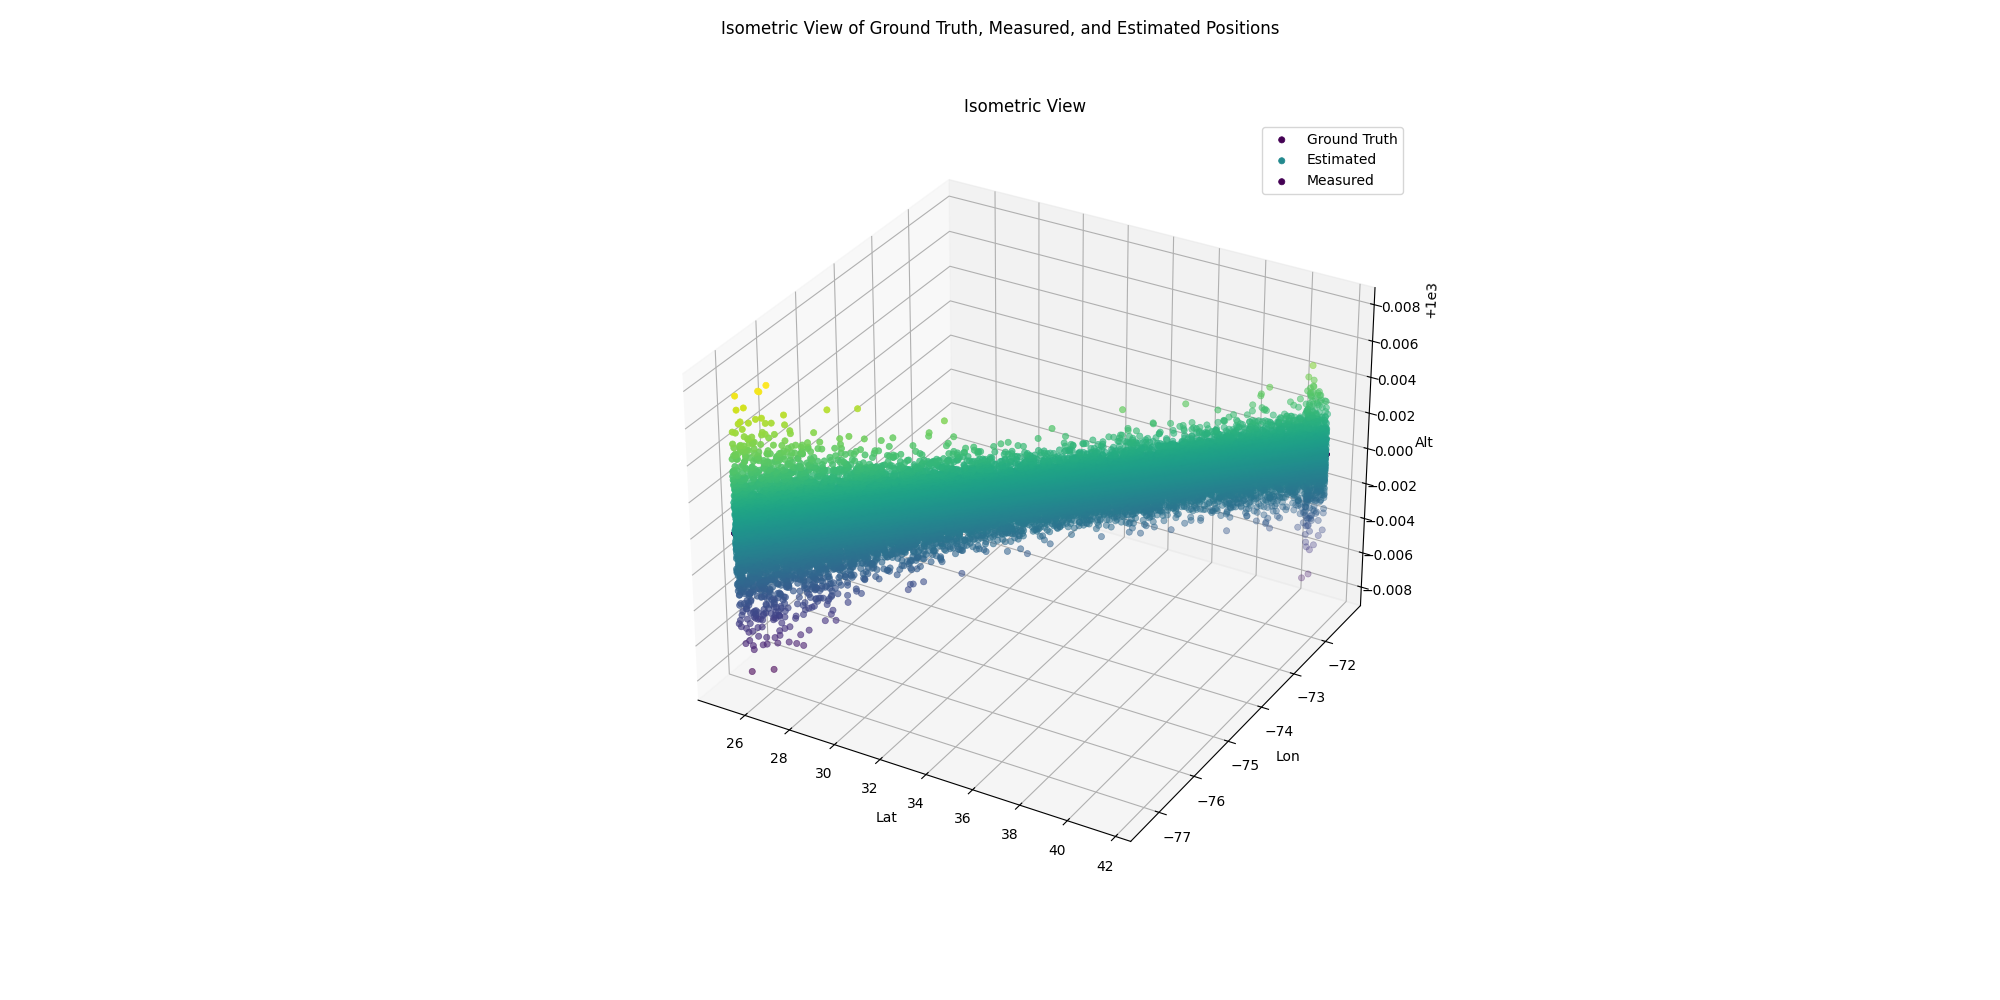
\includegraphics[width=0.8\textwidth]{./imgs/FB_isometric.png}
    \caption{Isometric View of the Feedback Model}
\end{figure}

Here we see the filter path overlayed on the ground truth path of that the aircraft took.

\begin{figure}[H]
    \centering
    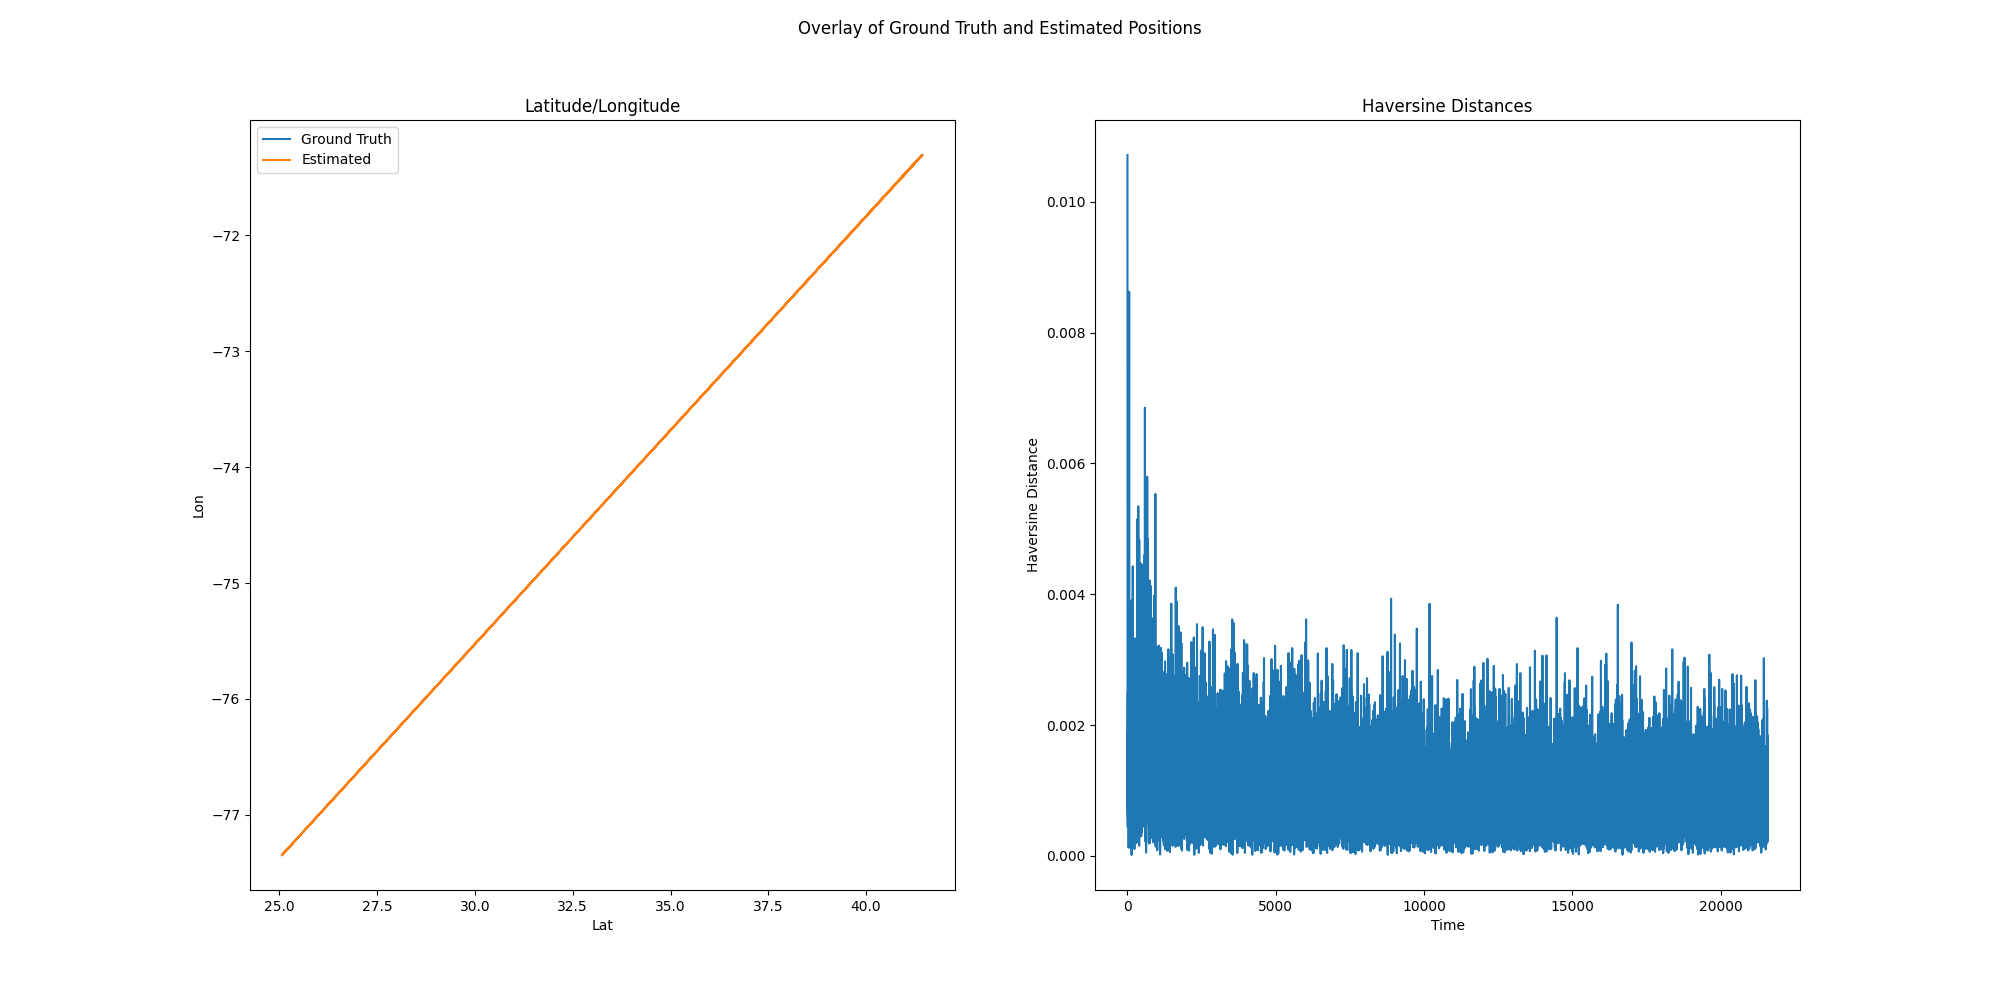
\includegraphics[width=0.8\textwidth]{./imgs/FB_latlon_haversines.png}
    \caption{Latitude/Longitude + Haversine Distance for the Feedback Model}
\end{figure}

Here we see the "overhead" view of the latitude and longitude of the aircraft during its path, with the faint sign of the ground truth path behind it. We also see a charting of the haversine distance of our expected position versus our estimated over time.

\begin{figure}[H]
    \centering
    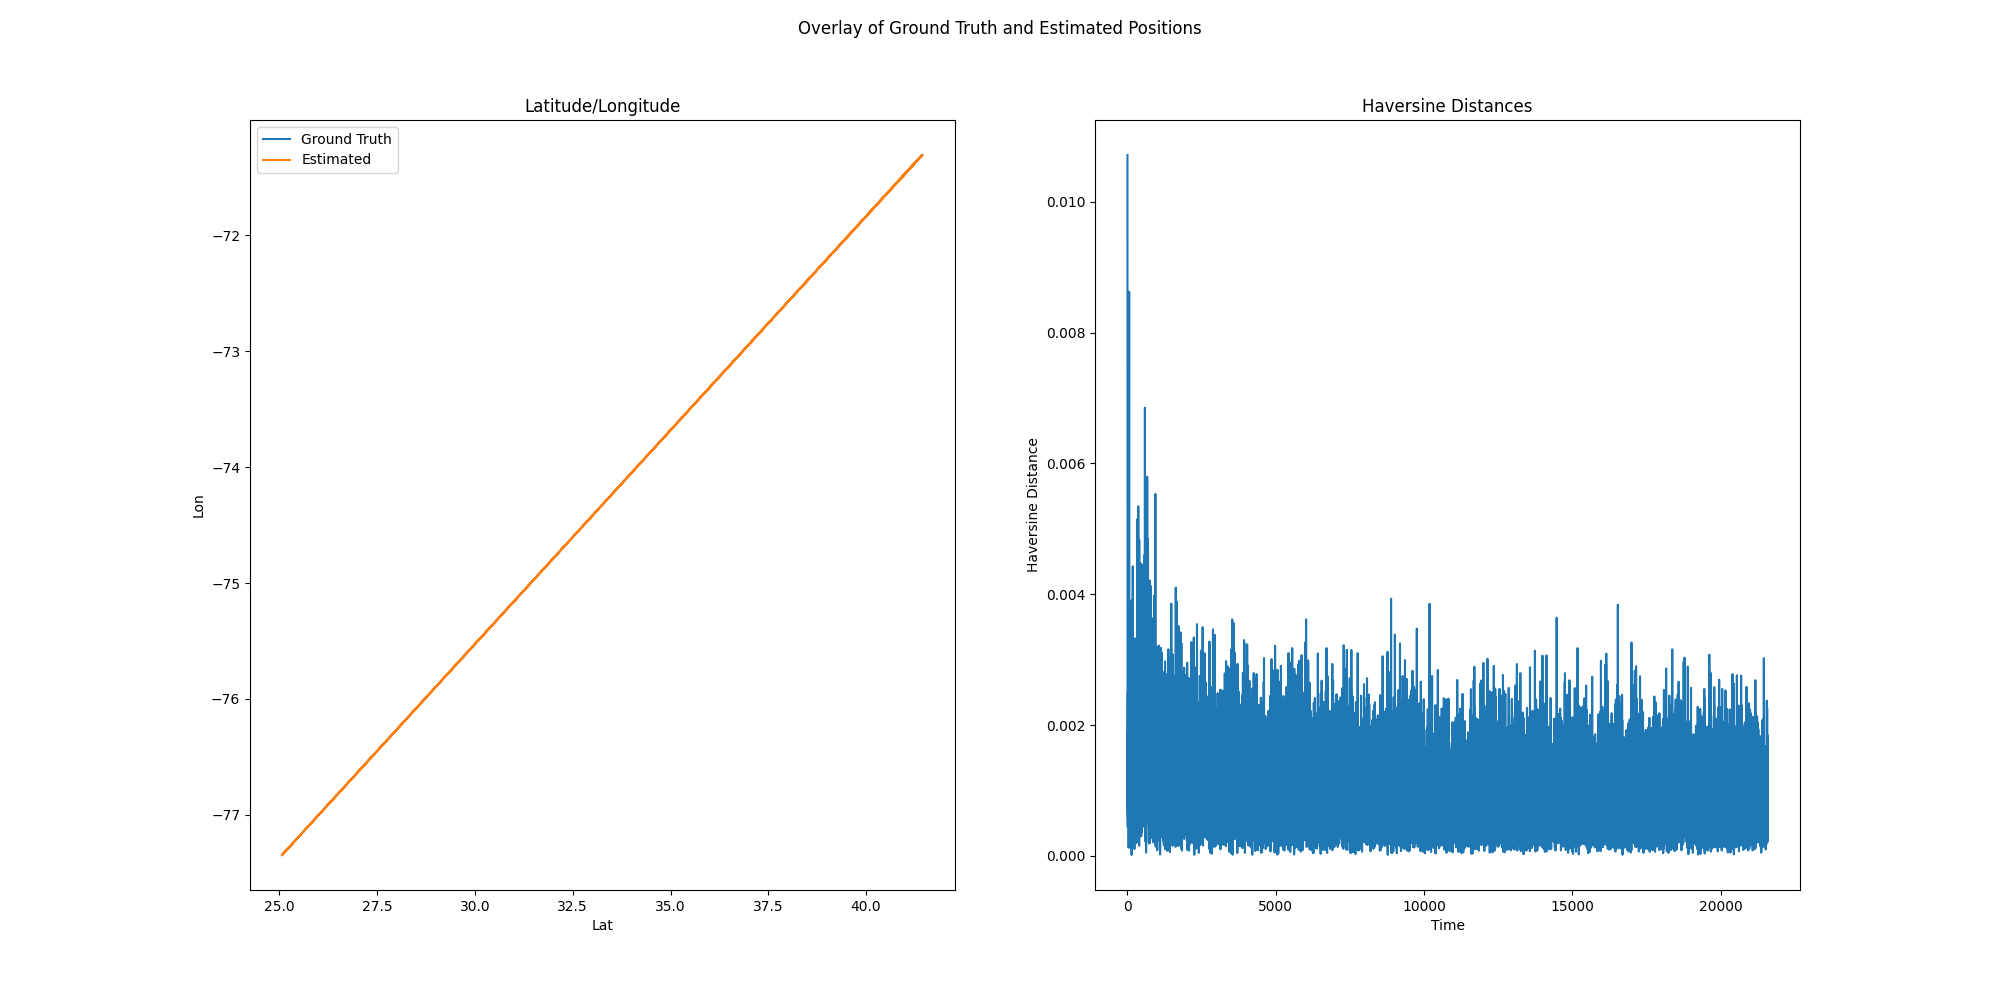
\includegraphics[width=0.8\textwidth]{./imgs/FB_statevar.png}
    \caption{State Variables for the Feedback Model}
\end{figure}

Here we see the individual state variables over time for the feedback model, with our ground truth projected underneath. This covers the latitude, longitude, altitude, roll, pitch, and yaw of our system over time.

\begin{figure}[H]
    \centering
    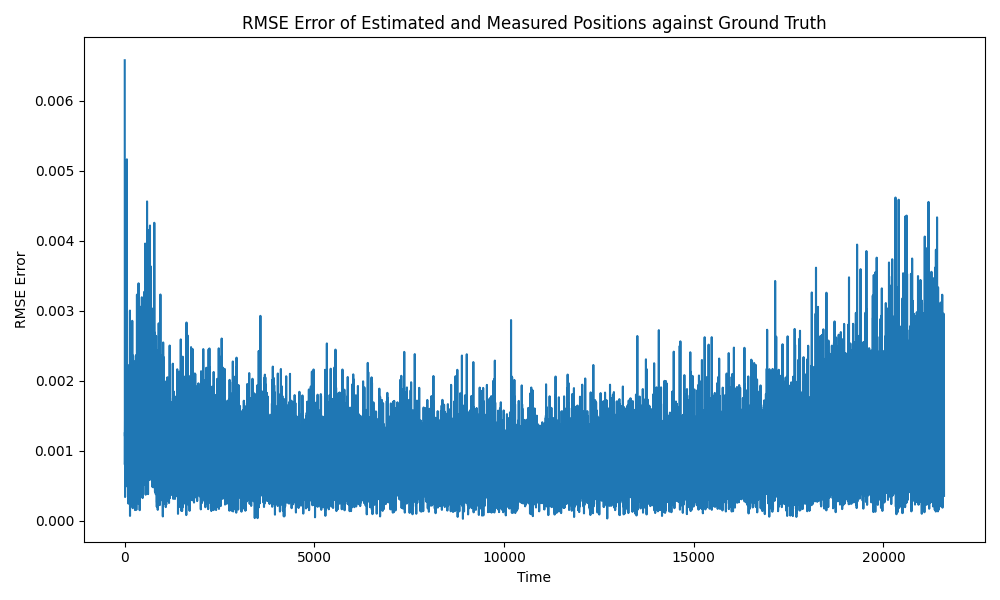
\includegraphics[width=0.8\textwidth]{./imgs/FB_rmse.png}
    \caption{RMSE for the Feedback Model}
\end{figure}

Here we see the calculated RMSE error of our positional estimation from the feedback filter over time. We see that while we have some spikes, our error is generally low at around $2.5\times10^{-3}$.

\subsection*{Feed Forward Model}

We now cover the feed forward model, which this author believes has an implementation issue, but still works:

\begin{figure}[H]
    \centering
    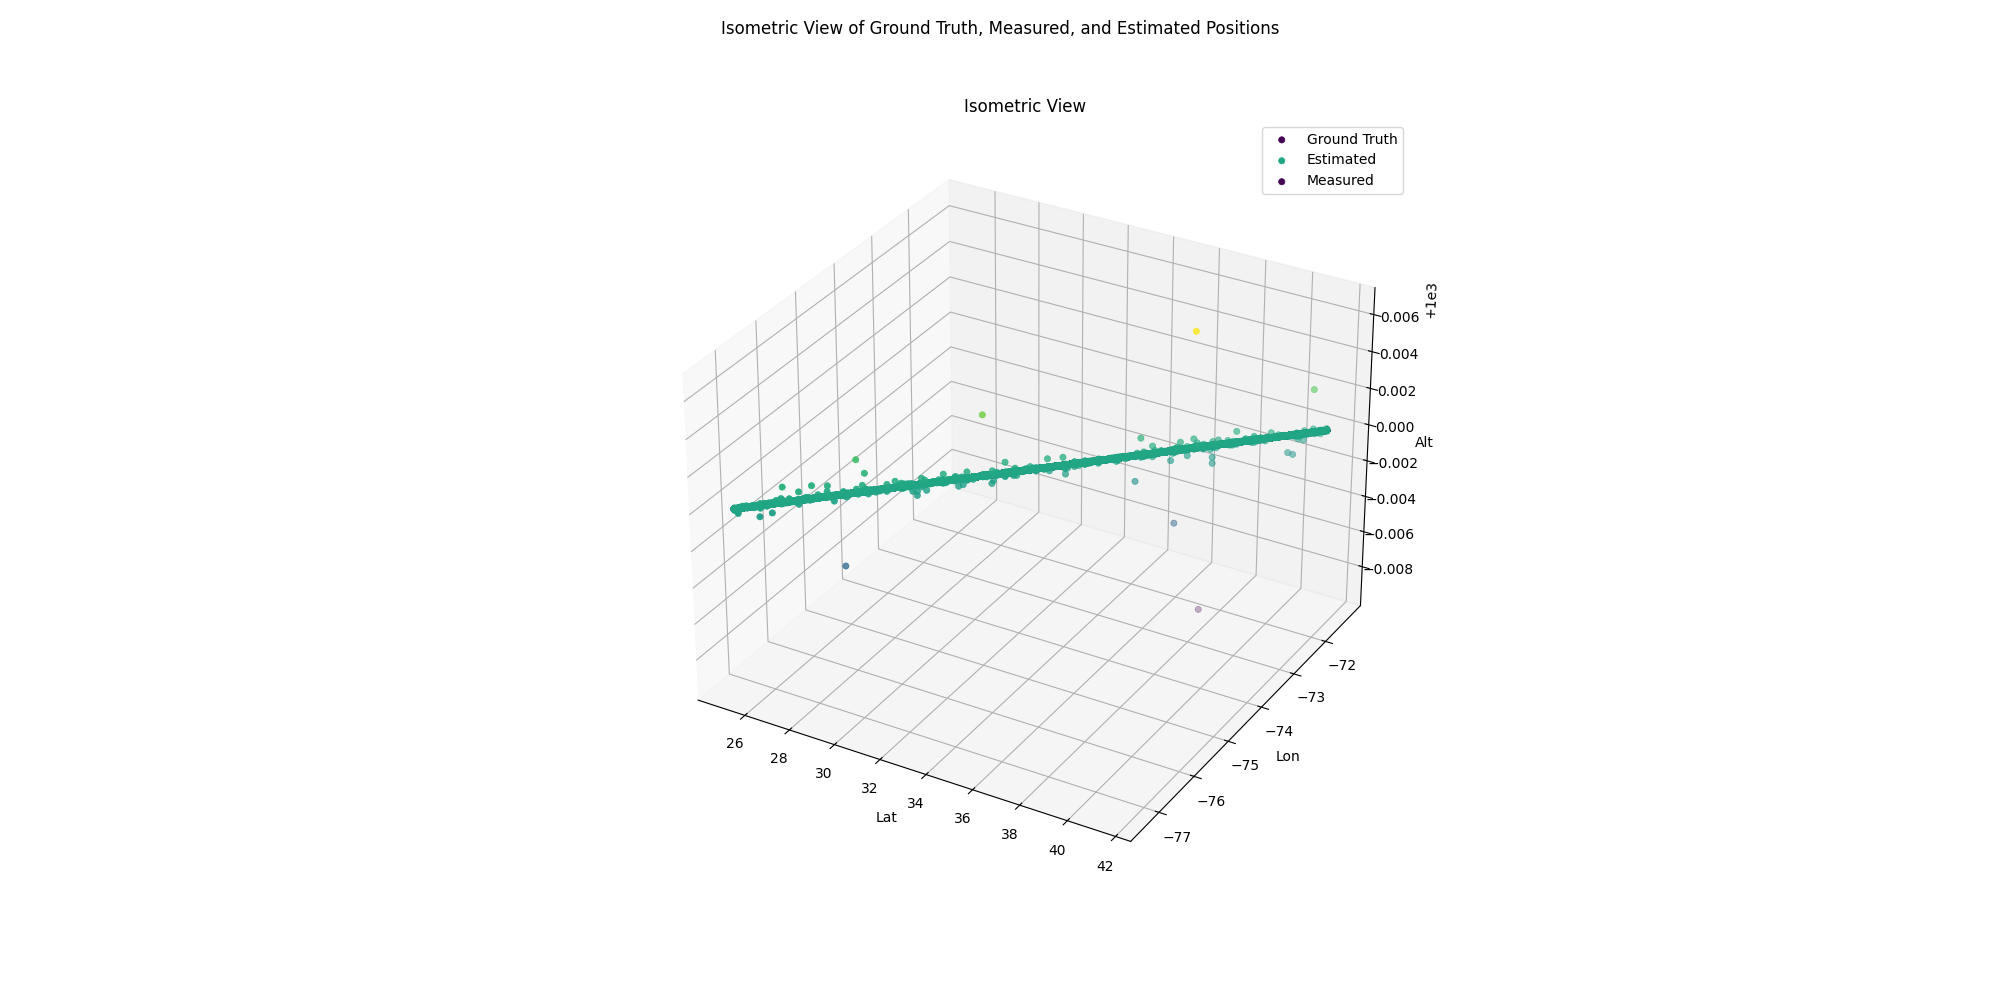
\includegraphics[width=0.8\textwidth]{./imgs/FF_isometric.png}
    \caption{Isometric View of the Feed Forward Model}
\end{figure}

Here we see the filter path overlayed on the ground truth path of that the aircraft took.

\begin{figure}[H]
    \centering
    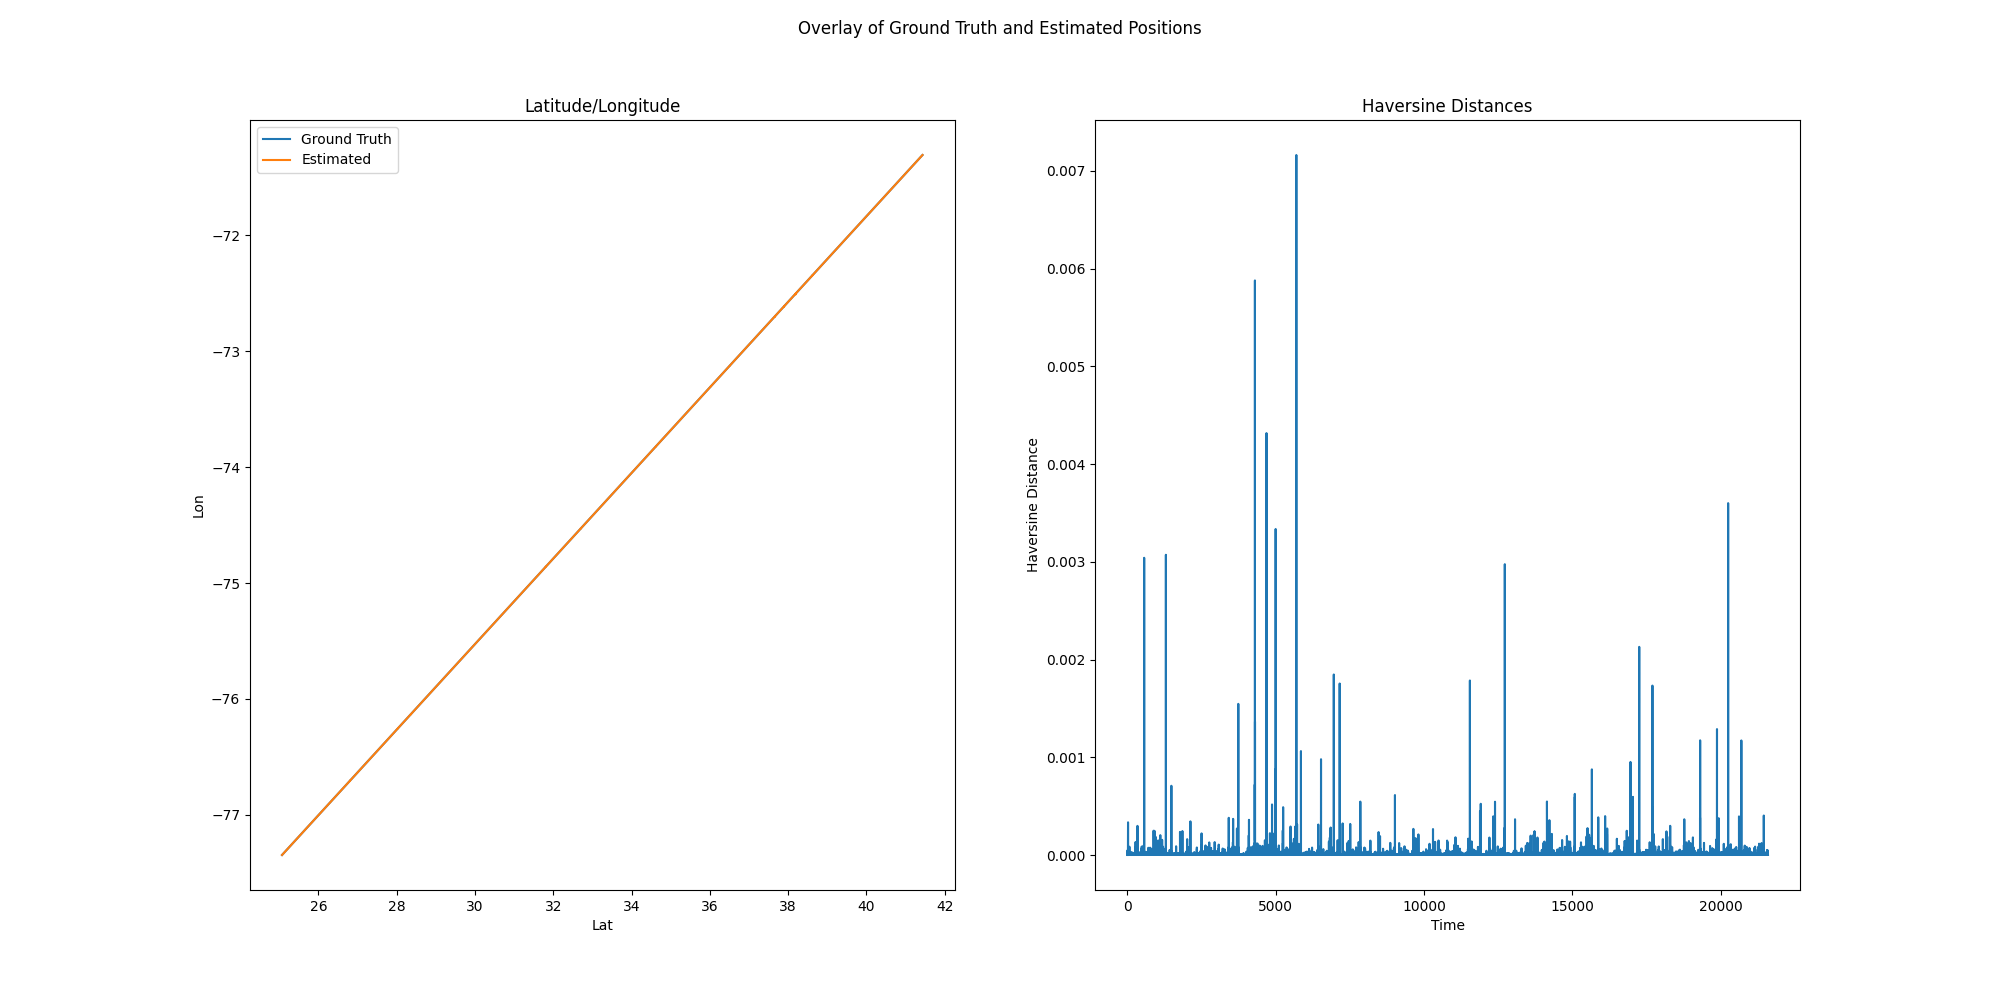
\includegraphics[width=0.8\textwidth]{./imgs/FF_latlon_haversines.png}
    \caption{Latitude/Longitude + Haversine Distance for the Feed Forward Model}
\end{figure}

Here we see the "overhead" view of the latitude and longitude of the aircraft during its path, with the faint sign of the ground truth path behind it. We also see a charting of the haversine distance of our expected position versus our estimated over time. We can see the haversine distances are noticeably higher than the FB model.

\begin{figure}[H]
    \centering
    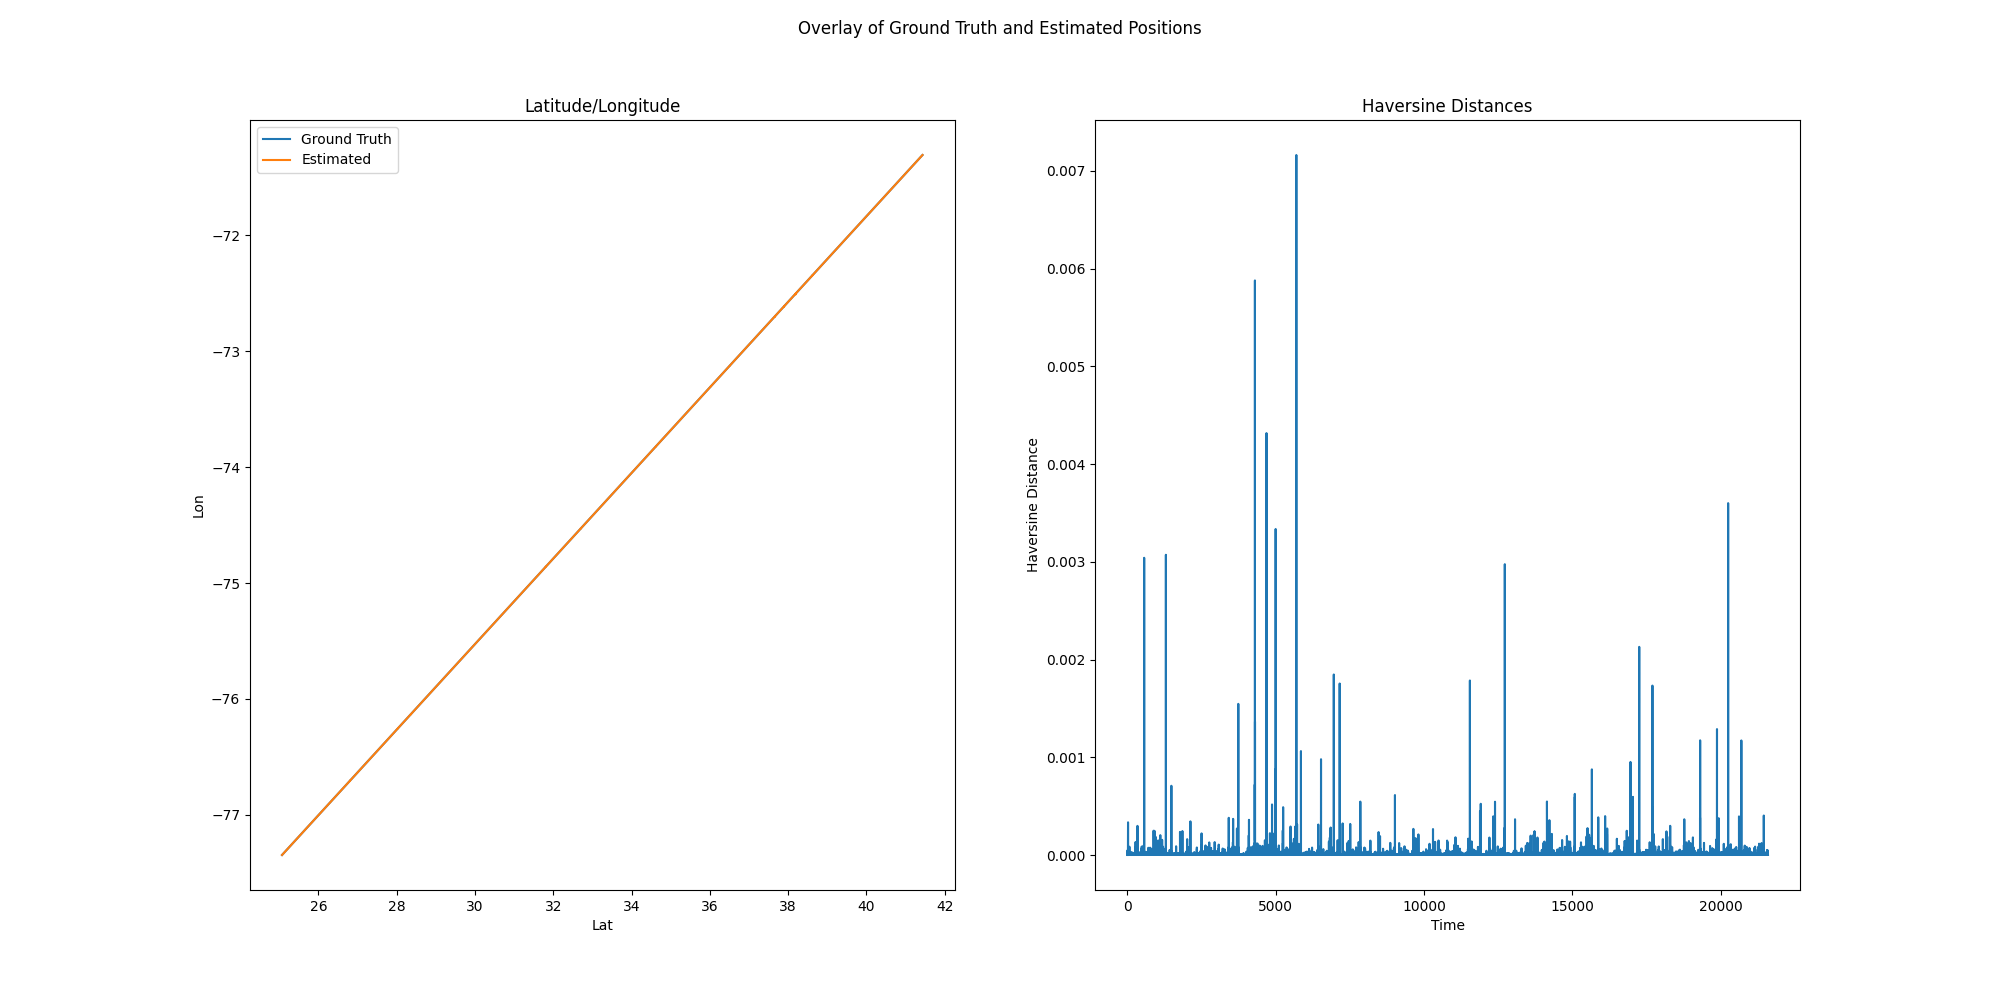
\includegraphics[width=0.8\textwidth]{./imgs/FF_statevar.png}
    \caption{State Variables for the Feed Forward Model}
\end{figure}

Here we see the individual state variables over time for the feed forward model. Again we see some spikes of instability that cause results to seem skewed that we did not see in the FB model.

\begin{figure}[H]
    \centering
    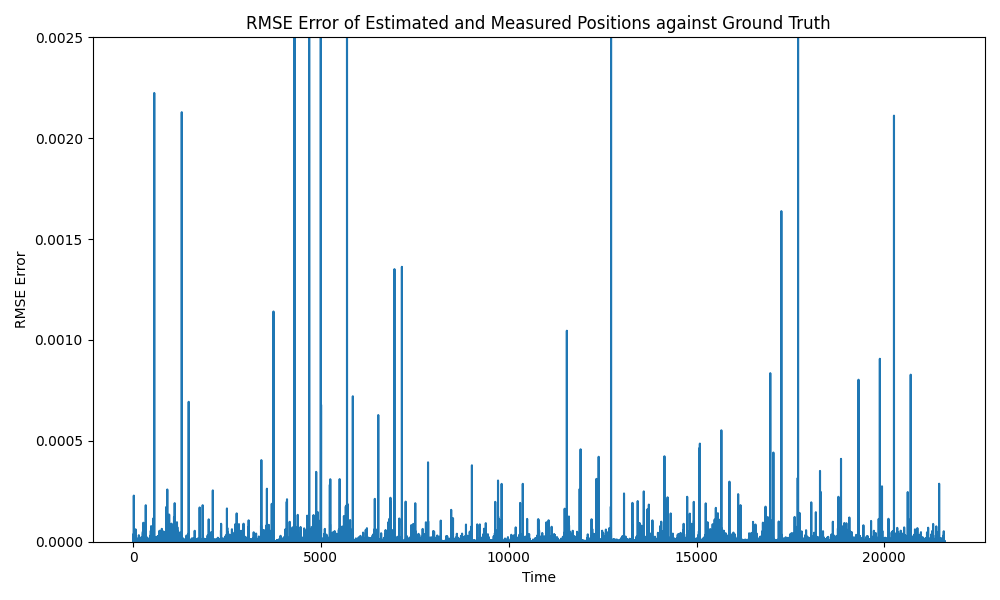
\includegraphics[width=0.8\textwidth]{./imgs/FF_rmse.png}
    \caption{RMSE for the Feed Forward Model}
\end{figure}

Finally, we see the calculated RMSE error of our positional estimation from the feed forward filter over time. We see an average error close to before, at around $3.5\times10^{-3}$, but we see huge spikes of error due to those aforementioned instability spikes.

\subsection*{Discussion}

The feedback model outperformed the feedforward method. This author expected the feedforward method to be more accurate, since the system considering the error and incorporating it into its estimations should create a more accurate model overall. However, this author believes they have an issue in the implementation somewhere, wherein they are introducing an inaccurate calculation of the covariance matrix to be a non positive definite matrix, causing issues down stream. To adjust this, we introduced a jitter fix method found within the \textit{fix\_covariance} recursive method, wherein we add increasing amounts of jitter noise to knock the generated covariance matrix back to positive definite. This works, but likely introduces downstreams effects to accuracy.

If we were tasked with improving this system, we would likely want to introduce some additional method to provide a loop closure in our localization of the plane, from which we can introduce "resets" of a known position and extrapolate from there, preventing error from building over the time of the flight and creating untenable situations in navigation guidance.

\end{document}